
%% Template Elsevier for Neuroimage

%% Use the option review to obtain double line spacing
%\documentclass[authoryear,preprint,review]{elsarticle}
\documentclass[authoryear]{elsarticle}
%\usepackage[framed,numbered,autolinebreaks,useliterate]{mcode}
\usepackage[framed,autolinebreaks,useliterate]{mcode}
\usepackage{natbib}
\usepackage{amsmath}
%\usepackage{lineno}
\usepackage{rotating}

\usepackage{hyperref}
\usepackage{amssymb}
\usepackage{amsfonts}


%\usepackage{algorithm2e}
%\usepackage{algorithmic}
%\usepackage{todonotes}
\usepackage{pdflscape}
\journal{Neuroimage}
\usepackage{color,transparent}
%\usepackage{color} 
%\pdfoptionpdfminorversion 6
\pdfminorversion=5

%\usepackage{graphicx}
%\usepackage{subcaption}
%\usepackage{mwe}
\usepackage{subfig}
\usepackage{caption}
%\usepackage{subcaption}
\usepackage{setspace}

\begin{document}

% Title must be 150 words or less
\begin{frontmatter}
%\title{Feasibility of multi-centric fMRI connectivity studies of Alzheimer's disease}
%\title{Feasibility of multi-centric fMRI connectivity and impact }

%\title{Measurement bias and statistical power in multi-centric resting-state fMRI connectivity}
\title{Statistical power and measurement bias in multi-centric resting-state fMRI connectivity}


%\title{A power analysis for multisite studies in resting-state functional connectivity, with an application to clinical trials in Alzheimer's disease}

\author[a,b]{Christian~Dansereau}
\author[c]{Celine~Risterucci}
\author[c]{Emilio~Merlo Pich}
\author[d]{Douglas~Arnold}
\author[a,b]{Pierre~Bellec\corref{cor1}}
\ead{pierre.bellec@criugm.qc.ca}
\cortext[cor1]{Corresponding author}
\address[a]{Centre de Recherche de l'Institut Universitaire de G\'eriatrie de Montr\'eal, Montr\'eal, CA}
\address[b]{D\'epartement d'Informatique et de recherche op\'erationnelle, Universit\'e de Montr\'eal, Montr\'eal,CA}
\address[c]{F. Hoffmann-La Roche Ldt., Basel, Switzerland}
\address[d]{NeuroRx, Montreal, Quebec, Canada}

% Please keep the abstract between 250 and 300 words
\begin{abstract}


\end{abstract}

%-- 
\begin{keyword}
multisite \sep multiprotocol \sep bias \sep statistical power \sep sample size \sep resting-state \sep fMRI, connectivity
%fmri \sep effect size \sep multisite \sep clinical trial \sep AD biomarker
\end{keyword}
\end{frontmatter}

% Unique number for each line
%\linenumbers
%\listoftodos

\section*{Highlights}

\begin{itemize}
\item etc
 %\item The impact of the number of nodes, or scale, on the sensitivity of a connectome-wide association study is systematically evaluated.
 %\item A procedure is presented that controls the false-discovery rate within- and between scales.
 %\item The technique is evaluated on a simulation of multiscale changes in connectome organization.
 %\item The technique is applied on three different datasets, for which there is a good a priori knowledge on the underlying connectivity changes.
 %\item Several recent procedures for connectome-wide association are compared.
\end{itemize}

\section{Introduction}

% Magic paragraph
\paragraph{Main objective}
Studies collecting brain images at multiple sites are becoming increasingly common in resting-state functional magnetic resonance imaging (rs-fMRI). In particular, some consortia have retrospectively shared rs-fMRI data from multiple independent studies of comparable populations, with the objective of dramatically increasing the sample size at the cost of decreased sample homogeneity, e.g. normal controls in the 1000 functional connectome project (FCP) \citep{Biswal2010}, children and adolescents suffering from attention deficit hyperactivity disorder from the ADHD200 \citep{ADHD200,Fair2012}, or individual diagnosed with autism spectrum disorder in ABIDE \citep{Nielsen2013}. Recruitment of patient populations in a limited time frame may also require acquisitions at multiple sites, e.g. the Alzheimer’s disease neuroimaging initiative (ADNI) \citep{Mueller2005} (REF2) fBIRN \citep{Friedman2006,Friedman2006a}, which is a common practice in pharmaceutical clinical trials at phase II and III \footnote{\url{http://www.roche-trials.com/trialDetailsGet.action?studyNumber=BP28248}}. An important benefit of multisite acquisitions is to offer improved generalization compared to single site studies, due to more diversity in scanners and populations. These additional sources of variance may however decrease the statistical power, and somewhat mitigate the benefits of having a large sample size. In this work, our main objective was to quantitatively assess the impact of inter-site variability on statistical power, for rs-fMRI group comparison.

\paragraph{Statistical power}
A simple and popular measure of individual resting-state connectivity is the Pearson’s correlation coefficient between the average temporal rs-fMRI fluctuations of two brain parcels. To compare two groups, a general linear model (GLM) is typically used to establish statistical difference in average connectivity between the groups, while accounting for possible confounding variables such as age, sex or the amount of head motion during the scan. Based on the parameters estimated by the GLM, a p-value is generated for each connection to quantify the probability that the difference in average connectivity is significantly distant from zero \citep{Worsley1995}. If the estimated p-value is smaller than a prescribed false-positive rate, say $\alpha=0.05$, then the difference in connectivity is deemed significant. Although in classical statistical testing the statistical decision is made purely based on the p-value, or type I errors, the statistical power is as critical as it controls for type II errors, i.e. failing to detect true differences. The statistical power is defined as the probability of finding a significant difference, when there is indeed a true difference. In the GLM, the statistical power in addition to sample size \citep{Desmond2002}: (1) the sample size; (2) the absolute size of the effect, i.e. the difference in mean connectivity between groups; and, (3) the variability of measures. 
The careful design of a study typically involves selecting the sample size in order to achieve a reasonable statistical power, say larger than $80\%$. But the choice of a multisite vs monosite study design may also impact statistical power by increasing the variability of measures. The recent work of \cite{Yang2014} have shown the presence of a significant bias in rs-fMRI measures between site, yet, to the best of our knowledge, the amplitude of this bias and its implications for statistical power calculation are not currently documented in the literature. 

\paragraph{Sources of variance in rs-fMRI}
The variability of rs-fMRI connectivity measures has both physiological and instrumental origins. Some sources of variability are shared by monosite and multisite studies, while others are specific of multisite studies. We can first note that rs-fMRI connectivity only has moderate-to-good test-rest reliability, when the measure is repeated for the same subjects in the same scanner \citep{Shehzad2009}. Many physiological factors likely contribute to these variations, such as the cognitive state of the subject, the level of alertness/drowsiness, circadian rhythm, hunger, medical regimen, potential neurostimulants, amongst others. There is also an instrumental variability even within subject and within scanner. The thermal noise in rs-fMRI only has a small amplitude (REF), but there are non-uniformity artefacts which have a strong impact on the signal, and will vary from session to session with the positioning of subjects as well as the adjustment of shimming (REF). Another source of within-site variations is the difference in connectivity across subjects. These variations are substantial and have been associated to a myriad of variables and clinical conditions (REF review). Taken together, the combination of within- and between-subjects variance is expected to have a large amplitude even at a single site. Multisite studies will add additional sources of physiological variations, as populations at different sites may substantially differ in terms of ethnicity, language, diet, socioeconomic status, exposure to pollutants, typical medication, quality of health services, etc. Some of these factors will be present even if stringent and harmonized inclusion/exclusion criteria are applied, e.g. diet or language. In terms of instrumentation, the fMRI measurements across sites can be affected by the scanner make and model \citep{Friedman2006}, sequence parameters such as repetition time, flip angle, or acquisition volume \citep{Friedman2006a}, experimental design such as eyes-open/eyes-closed \citep{Yan2009} or experiment duration \citep{VanDijk2010}, and scanning environment such as sound attenuation measures \citep{Elliott1999}, room temperature \citep{Vanhoutte2006}, or head-motion restraint techniques \citep{Edward2000}. Many of these parameters can be harmonized to some extent, but some differences may always remain, e.g. even identical scanners may have different software versions or upgrades.

\paragraph{Specific objectives}
To establish the impact of multisite acquisitions on statistical power in rs-fMRI, we first specifically aimed at characterizing the amplitude of the inter-site bias in real rs-fMRI measures, relative to intra-site variance. We based our evaluation on N=345 young healthy participants from the 1000 Functional Connectomes Project (FCP), including rs-fMRI samples independently collected at 8 imaging sites with 3T scanners in Germany, the United Kingdom, Australia and the United States of America. Datasets in this study were shared retrospectively and every documented parameters of image acquisition varied across studies. This data sample thus represents a worst-case-scenario in terms of 3T instrumental inter-site variations. Our second specific aim was to evaluate the impact of such inter-site bias on the detection power of rs-fMRI group comparison, in relation with sample size, group balancing and interaction between sites and group differences. We implemented for this purpose a series of simulation, mixing synthetic data with real data from the 1000 FCP. One of the particularity of the 1000 FCP is the presence of one large site of $\sim200$ subjects and 7 small sites of $\sim20$ subjects per site. We were therefore able to implement realistic scenarios following either a monosite or a multisite design, with the same total sample size.

\section{Method}

\subsection{Data samples} 

\paragraph{Participants}
The paper studies 345 cognitively normal young adults (CNY) from the 1000 functional connectome project\footnote{\url{http://fcon_1000.projects.nitrc.org/}} (150 males, age range = 18-46 yrs) as a reference dataset. One of the particularity of this dataset is the presence of one large site of $\sim200$ subjects and 7 small sites of $\sim20$ subjects per site. We are therefore able to simulate realistic scenarios where we model the variability of a real monosite and the variability introduced by combining small sites into a large sample of the same total sample size, see Table \ref{table_dataset} for more details on each site. The experimental protocols for all datasets were approved by there respective ethic boards.


\begin{table}[tbp]
\resizebox{\columnwidth}{!}{%
\begin{tabular}{lllllllllll}
\textbf{Site}         & \textbf{Magnet} & \textbf{Scaner brand} & \textbf{Channels} & \textbf{N} & \textbf{N final} & \textbf{Sex} & \textbf{Age} & \textbf{TR} & \textbf{\# Slices} & \textbf{\# Frames} \\
Baltimore, USA        & 3T              & N/A                   & N/A               & 23   & 21         & 8M/15F       & 20-40        & 2.5         & 47                 & 123                \\
Berlin, Germany       & 3T              & Siemens Tim Trio      & 12                & 26   & 26         & 13M/13F      & 23-44        & 2.3         & 34                 & 195                \\
Cambridge, USA        & 3T              & Siemens Tim Trio      & 12                & 198  & 195        & 75M/123F     & 18-30        & 3           & 47                 & 119                \\
Newark, USA           & 3T              & N/A                   & N/A               & 19   & 17         & 9M/10F       & 21-39        & 2           & 32                 & 135                \\
NewYork\_b, USA       & 3T              & Siemens               & N/A               & 20   & 18         & 8M/12F       & 18-46        & 2           & 33                 & 175                \\
Oxford, UK            & 3T              & Siemens Tim Trio      & 12                & 22   & 20         & 12M/10F      & 20-35        & 2           & 34                 & 175                \\
Queensland, Australia & 4T              & Bruker                & 1                 & 19   & 17         & 11M/8F       & 20-34        & 2.1         & 36                 & 190                \\
SaintLouis, USA       & 3T              & Siemens Tim Trio      & 12                & 31   & 31         & 14M/17F      & 21-29        & 2.5         & 32                 & 127               
\end{tabular}
}
\caption{Site selected from the 1000 functional connectome dataset.} 
\label{table_dataset}
\end{table}

\paragraph{Acquisition} %Resting-state scans were acquired on a 3T Siemens TrioTim for all datasets. One single run was obtained per subject for either the SCHIZO or BLIND dataset while two runs were acquired in each subject for the MOTOR dataset, one immediately preceding and one following the practice on a motor task. 
%For the 1000 functional connectom dataset, 150 EPI volumes were recorded in 6 mins 40 s (TR = 2.65s, TE = 30ms, FA = 90\textdegree, 43 slices, voxel size = 3.4x3.4x3 mm$^3$, gap = 10\%, matrix size = 64x64, FOV = 220x220 mm$^2$), and a structural image was acquired using a MPRAGE sequence (TR = 2.3~s, TE = 2.98~ms, FA = 9\textdegree, 176 slices, voxel size = 1x1x1 mm$^3$, matrix size = 256x256, FOV = 256x256 mm$^2$).

We need to discuss how to present this data (I don't have the details for each site...)

\subsection{Preprocessing}\label{Preprocessing}
The datasets were analysed using the NeuroImaging Analysis Kit (NIAK\footnote{\url{http://www.nitrc.org/projects/niak/}}) version 0.12.14, under CentOS version 6.3 with Octave\footnote{\url{http://gnu.octave.org}} version 3.8.1 and the Minc toolkit\footnote{\url{http://www.bic.mni.mcgill.ca/ServicesSoftware/ServicesSoftwareMincToolKit}} version 0.3.18. Analyses were executed in parallel on the "Mammouth" supercomputer\footnote{\url{http://www.calculquebec.ca/index.php/en/resources/compute-servers/mammouth-parallele-ii}}, using the pipeline system for Octave and Matlab \citep{Bellec2010}, version 1.0.2. Brain map visualizations were created using MRICron software \cite{Rorden2007}. Each fMRI dataset was corrected of inter-slice difference in acquisition time and the parameters of a rigid-body motion was estimated for each time frame. Rigid-body motion was estimated within as well as between runs, using the median volume of the first run as a target. The median volume of one selected fMRI run for each subject 
was 
coregistered with a T1 individual scan using Minctracc \citep{Collins1998}, which was itself non-linearly transformed to the Montreal Neurological Institute (MNI) template \citep{Fonov2011} using the CIVET pipeline \citep{Zijdenbos2002}. The MNI symmetric template was generated from the ICBM152 sample of 152 young adults, after 40 iterations of non-linear coregistration. The rigid-body transform, fMRI-to-T1 transform and T1-to-stereotaxic transform were all combined, and the functional volumes were resampled in the MNI space at a 3 mm isotropic resolution. A censoring method described in \citep{Power2012} called "scrubbing" was used to remove the volumes with excessive motion using a cut-off value of $FD\geq0.5$. A minimum number of 50 unscrubbed volumes per run, corresponding to $\sim 125$ s of acquisition for a TR of 2.5 seconds, was then required for further analysis. The following nuisance parameters were regressed out from the time series at each voxel: slow time drifts (basis of discrete cosines 
with a 0.01 Hz high-pass cut-off), average signals in conservative masks of the white matter and the lateral ventricles as well as the first principal components (95\% energy) of the six rigid-body motion parameters and their squares \citep{Lund2006},\citep{Giove2009}. The fMRI volumes were finally spatially smoothed with a 6 mm isotropic Gaussian blurring kernel. 


\subsection{Functional networks}

\paragraph{Functional parcellation}
Regions are routinely defined using an anatomical parcellation \citep{He2009}, such as the AAL template \citep{Tzourio-Mazoyer2002}. Anatomical parcels may however not well match the brain functional organization. In this work, we used functional brain parcellations, aimed at defining groups of brain regions with homogeneous time series. A number of algorithms have been proposed with additional spatial constraints, to ensure that the resulting parcels are spatially connected \citep{Lu2003,Thirion2006,Craddock2012}. We can achieve this aim and reduce the computational burden of the analysis using a region-growing algorithm \cite{Bellec2006},  resulting in more homogeneous regions composed of temporally similar and contiguous voxels. The spatial dimension was selected arbitrarily by setting the size where the growing process stopped (a threshold of 1000 mm3 resulted into R=957 regions) from a reference dataset of healthy adults from the 1000 functional connectome project (Cambridge cohort \citep{Biswal2010}, parcellation available here \ref{}). The regions were built to maximize the homogeneity of the time series within the region, i.e. the average correlation between the time series associated with any pair of voxels of the region. The region growing was applied on the time series concatenated across all subjects (after correction to zero mean and unit variance), such that the homogeneity was maximized on average for all subjects, and the small homogeneous regions are identical for all subjects. Because of the temporal concatenation of time series, we had to limit the memory demand, and the region-growing was thus applied independently in each of the 116 areas of the AAL template \citep{Tzourio-Mazoyer2002}. See \cite{Bellec2006} for more details regarding the implementation of the region-growing algorithm. Overall, this process reduced the dataset of each subject into a (T x R) data array, where T is the number of time samples and R is the number of regions.

\paragraph{Functional network decomposition}
From a pure functional viewpoint, the spatial constraint seems somewhat arbitrary, as functional units in the brain at low resolution encompass distributed networks of brain regions with homotopic regions often being part of a single parcel \citep{DeLuca2006,Damoiseaux2006}. Some works have thus used distributed parcels as the spatial units to measure functional brain connectivity, e.g. \citep{Jafri2007,Marrelec2008}. We relied on a recent method called “Bootstrap Analysis of Stable Clusters” (BASC), which can identify consistent functional networks for a group of subjects \citep{Biswal2010}. using a hierarchical cluster with Ward’s criterion both at the individual and the group levels. The functional networks can be generated at any arbitrary scale (within the range of the fMRI resolution), and we considered only networks generated at the group level, which were non-overlapping and not necessarily spatially contiguous. In the present work we generated a BASC decomposition in 100 networks.

TODO: cite the NATURE paper of Pierre Orban for parcelation and connections selection.

\paragraph{Functional connectome}
Using a brain partition of $R$ networks obtain from BASC procedure described in \cite{Bellec2010c}, and taking each pair of distinct networks $i$ and $j$, the between-network connectivity $y_{i,j}$ is measured by the Fisher transform of the Pearson's correlation between the average time series of the network. The within-network connectivity $y_{i,i}$ is the Fisher transform of the average correlation between time series of every pair of distinct voxels inside network $i$. The connectome $\mathbf{Y}=(y_{i,j})_{i,j=1}^R$ is thus a $R\times R$ matrix. Each column $j$ (or row, as the matrix is symmetric) codes for the connectivity between network $j$ and all other brain networks (full brain functional connectivity map). For a scale with $R$ parcels, there are exactly $L=R(R+1)/2$ distinct elements in an individual connectome $\mathbf{Y}$.









\subsection{Simulations}

In order to simulate various scenarios within the context of a multi-site setting, a cohort of subjects acquired at a single-site was selected to act as our reference dataset and for the multi-site configuration a cohort from a collection of small sites, roughly totalling the same sample size as the reference dataset, was used. The simulation was based on a scenario with 8 sites for a total of 345 subjects, and no homogenization of acquisition protocol whatsoever. The multi-site (with correction) is based on 150 subjects from 7 sites and the monosite is based on one site of 195 subjects.  

\paragraph{Data generation process}
The following data generation model was used to test our hypothesis and estimate how the connectivity bias affect our ability to detect effects at the group level.
A sub-sampling procedure was performed on the datasets (monosite and multisite) previously described to obtain multiple samples ($B=10^3$ random samples). For each of the sample a Monte-Carlo simulation was implemented to evaluate the power of a resting-state multi-site study. For each site and each sample, a ratio $W$ of subjects were randomly assigned to a 'treatment' group, this ratio $W$ is referred to as the allocation ratio of participants. For the subjects in this group, a value was added to achieve a given relative effect size (Cohen's d, i.e. the mean of the two groups divided by the standard deviation of all sites, see Equation \ref{eq_cohen} for more details).

%Using sub-sampling it is possible to obtain an estimate of the mean statistical power over all samples which is call the detection power. These parameter estimates can then be used in simulation experiments to generate power curves.
%The detection power quantitatively express the reproducibility of the findings and we can therefore choose a sample size to achieve the desired detection power for a given probability of rejecting the null hypothesis.

\paragraph{Effect size (cohen's d)}
The normalized Cohen's d was used to estimate the effect size and it is defined as the difference between two means $\bar{x_{1}},\bar{x_{2}}$ divided by a standard deviation from the data $s$.

For each site an effect is added to the connectivity of $W$ of the subjects, selected randomly ("pathological" group):
\begin{equation}
	y_{i,j} = y_{i,j} + \mu.
\end{equation}

The parameter $\mu$ is chosen to obtain a particular effect size (measured by the Cohen $d$)
%The normalized Cohen's d was used to estimate the effect size and it is defined as the difference between two means $\bar{x_{1}},\bar{x_{2}}$ divided by a standard deviation from the data $s$.
\begin{equation}
\label{eq_cohen}
    \begin{array}{l l}
      d = \frac{\mu}{s_{i,j}},      
    \end{array}
\end{equation}
where $s_{i,j}$ is the standard deviation between region $i$ and $j$ for the reference population (mono-site). The significance of the difference between the control and 'treatment' group was assessed by a $t$-test in a linear model, including a covariate to model the motion. The study was repeated for various effect sizes (0 to 0.8 with a step of 0.01) with a $p$-value threshold of $0.001$ on the $t$-test.

In order to introduce the same effect-size across the single-site and multi-site dataset we are taking the standard deviation from the single-site cohort as the reference.  The connection $y_{i,j}$ of the randomly affected subjects ("treatment" group) are therefore calculated $y_{i,j} = y_{i,j} + d\times s_{i,j}$. 

\paragraph{GLM model} 
In order to detec changes on each connection pair between groups artificialy created population in each simulation, a general linear model (GLM) was performed and the following confounding variables were modelled in the analysis: age, sex and frame displacement (FD). To account for site-specific bias $S-1$ dummy-variables (binary vectors $1\times S$) were added to the model with $S$ being the total number of sites used in the study. The variables are corrected to have a zero mean across subjects, and an intercept (i.e. a column filled with 1) is added to $\mathbf{X}$ to capture the global average. The GLM relies on the following stochastic model Equation\ref{eq_glm_dummy}.

\begin{equation}
 \label{eq_glm_dummy}
  \mathbf{Y} = \mathbf{X}\mathbf{\beta} + \mathbf{V}\mathbf{\gamma}+ \mathbf{E},
\end{equation}
\begin{itemize}
  \item $\mathbf{Y}$: $N\times 1$, connectivity value for the pair ($i,j$),
  \item $\mathbf{X}$: $N\times K$, explainable variables,
  \item $\mathbf{\beta}$: $1 \times K$, regression values for each explainable variable,
  \item $\mathbf{V}$: $N\times S$, each column code for a site (0/1),
  \item $\mathbf{\gamma}$: $1\times S$, site average connectivity,
  \item $\mathbf{E}$: $N\times 1$, residual values from the regression,
\end{itemize}
 
with $N$ the number of subjects, $K$ the number of explainable variables and $S$ the number of sites. Where $\mathbf{\beta}$ is an unknown $1\times K$ vector of linear regression coefficients, $\mathbf{\gamma}$ is a $1\times S$ vector of linear regression coefficients representing the contribution of each site and $\mathbf{E}$ is a $N\times 1$ random (noise) multivariate Gaussian variable. As data generated from different subjects are statistically independent, and under an homoscedasticity assumption, the regression coefficients $\mathbf{\beta}$ can be estimated with ordinary least squares.

% statistical detection and sensitivity
\paragraph{Statistical detection and sensitivity}

We relied on the following parametric assumptions on the noise E (1) that its rows are independent; (2) that each element follows a normal distribution with zero mean, and (3) that the variance of all elements are constant within a column, also called the homoscedasticity assumptions. As the data generated from different subjects are statistically independent the first assumption is reasonable. We tested the normality and homoscedasticity assumptions on real datasets. Under these parametric assumptions, the regression coefficients $\mathbf{\beta}$ and $\mathbf{\gamma}$ can be estimated with ordinary least squares and, for a given “contrast” (difference between the control and 'treatment' group) the significance of the contrast is assessed by a Student $t$-test.

The sensitivity of the test was evaluated by the average detection performance of all the samples (see Equation \ref{eq_sensitivity}). For each sample $b$, we have a $p$-value $p^{*}_b$ and the detection sensitivity is estimated by the probability of $p^{*}_b$ being inferior to $0.001$.

\begin{equation}
    \frac{1}{B}\sum\limits_{b=1}^B\left(p^{*}_b\leq0.001\right).
    \label{eq_sensitivity}
\end{equation}



% The scenarios and the 3 sections
\paragraph{Simulations scenarios}

We first evaluated if a bias can be detected between sites. To do so we have computed the average connectome of each site along with the standard deviation matrix for each site. We then obtained a mask of the significant differences between each sites (Student $t-test$ corrected for multiple comparison using FDR $\alpha=0.05$) to have an idea of the size and spread of the functional bias.

For each experiment using real data, all effect size in the range 0 to 1.5 with a step of 0.01 were considered. The simulation were performed on 11 connections based on the literature review previously described in (TODO: cite the NATURE paper of Orban2015) reporting reproducible pair of regions reported to be affected by Alzheimer disease progression and displayed connectivity changes between cognitively normal subjects and patient with dementia of the Alzheimer type. We implemented a series of experiments:

\begin{itemize}
  \item We first checked how the total number of subject impact sensitivity using 3 different sample size (40, 80, 120) for an allocation ratio of $W=0.5$,
  \item We then checked how the allocation ratio of participants $W$ impact sensitivity using 3 different ratio ($W=0.5,0.3,0.15$) for a total sample size of 120,
  \item We checked how the allocation ratio of participants $W$ impact sensitivity using 3 different ratio ($W=0.5,0.3,0.15$) for a total sample size of 120, including an interaction site-pathology effect of $d=0.5$,
  \item We checked how the allocation ratio of participants $W=0.3$ impact sensitivity using only 2 sites one large (80 subjects) and one small ($\sim20$ subjects) instead of the 7 sites previously used,
\end{itemize}

%%%%%%%%%%%%%%%%%%%%%%%%%%%%%%%%%%%%%%%%%%%%%%%%%%%%%%
fully simulated data
In order to obtain more control on each of the parameter of the simulation and simulate some configuration that were not possible to do with the real data (like the simulation of 2 medium size sites of of 40 and 60 subjects per site, and the size of the site effect) we have therefore used a synthetic model using only synthetic data and the average standard deviation of the Cambridge site connectivity.

For each experiment using synthetic data, all effect size in the range 0 to 1.5 with a step of 0.01 were considered. The simulation were performed using randomly generated values. All experiments show four scenarios,  

For each experiment, all combinations of effect size in
the grid {without site-effect and with site-effect} and the grid {without interaction site-pathology and with interaction site-pathology} were considered. We implemented a series of experiments:

\begin{itemize}
  \item We first checked how 2 sites with respectively 50 subjects in each site with an allocation ratio of $W=0.5$ in both sites are impacted in the 4 scenarios in term of sensitivity,
  \item We then checked how 2 sites with respectively 50 subjects in each site with an allocation ratio of $W=0.7$ for the first site and $W=0.3$ for the second site are impacted in the 4 scenarios in term of sensitivity,
  \item We checked how 2 sites (one small of 20 subjects and one large of 80 subjects) with an allocation ratio of $W=0.5$ in both sites are impacted in the 4 scenarios in term of sensitivity,
  \item We checked how 2 sites (one small of 20 subjects and one large of 80 subjects) with an allocation ratio of $W=0.7$ for the first site and $W=0.3$ for the second site are impacted in the 4 scenarios in term of sensitivity,
   \item We checked how 2 sites (one small of 20 subjects and one large of 80 subjects) with an allocation ratio of $W=0.7$ for the first site and $W=0.3$ for the second site are impacted in the 4 scenarios in term of sensitivity,
   \item We checked how 50 sites (with a number of subject per site randomly assigned between 2 and 15) with an allocation ratio $W$ randomly assigned between 0.1 and 0.9 for each sites are impacted in term of sensitivity for 2 scenarios (without and with interaction site pathology),
\end{itemize}
 
 
\section{Results}

\subsection{Inter-site bias}
The first assessment perform on the dataset was to verify the distribution of the intra-site and inter-site functional connectivity variance to assess the magnitude of the bias. This analysis of Figure \ref{fig_site_variability} shows the distribution of the standard deviation in connectivity across subjects (the distribution is over the full brain connectome, with several 1000s connections) at the 8 sites against the inter-sites standard deviation of connectomes (average at each site). As we can see the inter-site (between-site) variability is smaller than the intra-site (between subjects) variability, in fact the amplitude of inter-site bias is about 3-fold smaller than the within-site standard deviation (red $\sim 0.06$ vs. orange $\sim 0.18$).

\begin{figure}[tbp]
\begin{center}
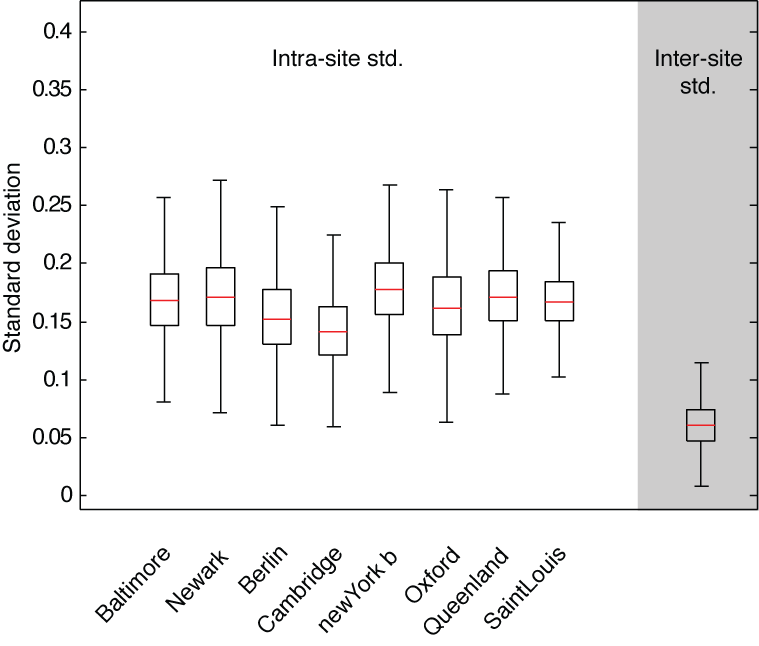
\includegraphics[width=\linewidth]{../figures/inter_vs_intra_3tonly.png}
\end{center}
\caption[inter vs. intra site variability]{
  Distribution of intra-site (between-subject) standard deviation vs. inter-site (between-site) standard deviation, based on the standard deviation of the connectivity matrices from 8 sites from the 1000 functional connectome dataset.
}
\label{fig_site_variability}
\end{figure}




In order to verify how spatial structure vary across sites the average standard deviation and the average connectivity map of the DMN were extracted for each site and reported in Figure \ref{fig_DMN_variability}. As we can see in the intersection between two sites the difference in average connectivity between-sites is illustrated (red set of brain cuts). First the mean DMN at each site is consistent with the expected spatial distribution reported in other studies \citep{Damoiseaux2006,Dansereau2014,Yan2013a}. The most salient changes between-sites are located in the mesio-frontal region associated with the anterior part of the DMN. In order to verify if significant changes are not only found in the DMN we have computed the entier connectome in order to obtain the other connectivity patterns and the findings can be generalized to the full connectome see Figure \ref{fig_connectome_variability}.

\begin{figure}[tbp]
\begin{center}
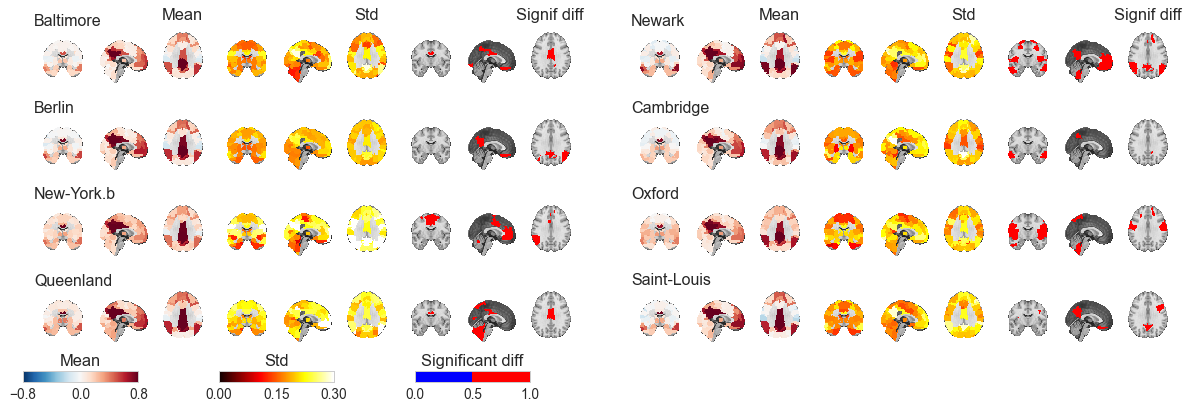
\includegraphics[width=\linewidth]{../figures/pccmap_multisite.png}
\end{center}
\caption[DMN variability across sites]{
Functional connectivity maps of the default-mode network at multiple sites. The average connectivity map are shown on the diagonal. The standard deviation across subjects and within site is shown on the first column. Each off-diagonal block represent the significant differences between the average functional connectivity maps between two sites (called the inter-site bias).
}
\label{fig_DMN_variability}
\end{figure}


\begin{figure}[tbp]
\begin{center}
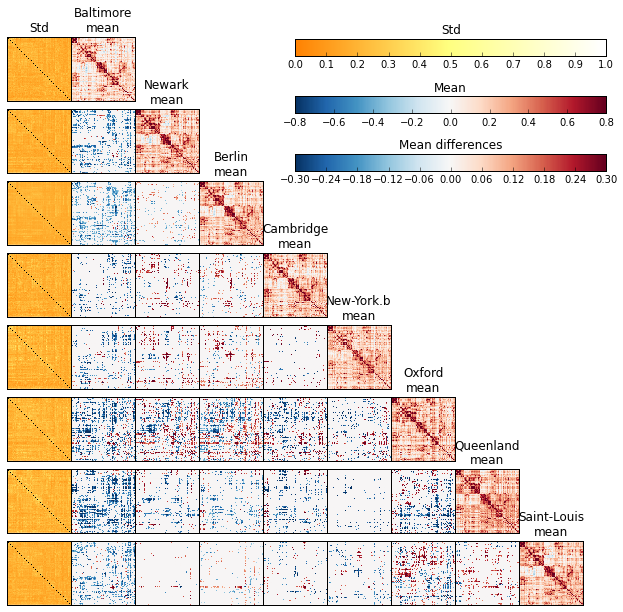
\includegraphics[width=\linewidth]{../figures/connectome_multisite.png}
\end{center}
\caption[Connectome variability across sites]{
Functional connectome for multiple sites. The average connectome of 8 sites (Baltimore, Newark, Berlin, Cambridge, New-Yorkb, Oxford, Queenland and SaintLouis at 3T) are shown on the diagonal. The standard deviation across subjects and within site is shown on the first column. Each off-diagonal block represent the absolute difference between the average functional connectivity maps between two sites (called the inter-site bias).
}
\label{fig_connectome_variability}
\end{figure}

\subsection{Simulation on real data}
% introduction of simulation intro the objectives...

In order to evaluate the impact of multisite configuration on our ability to detect changes in rs-functional connectivity studies we performed various simulation on real fMRI data. For each site and each sample, $B$ of the subjects were randomly assigned to a 'treatment' group. For the subjects in this group, a value was added to achieve a given relative effect size expressed in Cohen's d. The significance of the difference between the control and 'treatment' group was assessed by a $t$-test in a linear model. To account for site-specific bias we have included dummy variables in the GLM model. The study was repeated for various effect sizes (0 to 1.5 with a step of 0.01) at a threshold of 0.001 on the p-value.

Figure \ref{fig_p2p} show the pair of regions used in (TODO ORBAN2015) as candidate marker for functional connectivity changes in Alzheimer disease based on a literature review. We will use the correlation between those regions to estimate the variability across subject and induce some effect in our simulations.

\begin{figure}[tbp]
\begin{center}
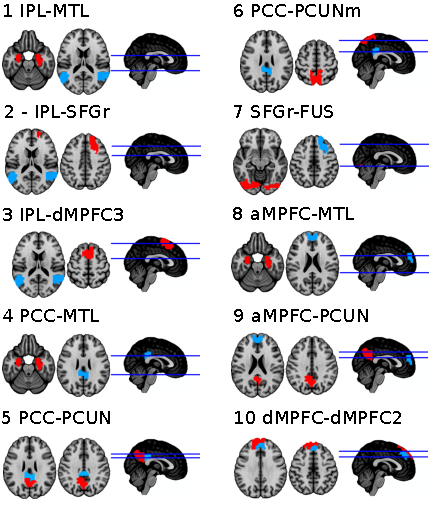
\includegraphics[width=0.5\linewidth]{../figures/p2p_seeds.pdf}
\end{center}
\caption{
Connexions pair based on a literature review.
}
\label{fig_p2p}
\end{figure}


In Figure \ref{fig_real_sim_samplesize} we show the effect of the sample size on the detection power. As expected we are able to detect smaller and smaller effect size as we increase the sample size. For an effect size of 1 which is considered a large effect we are able to detect significant changes in only 20\% of the cases at 40 subjects, 80\% at 80 subjects and almost 95\% at 120\% subjects. The statistical power is at p<0.001.

%\frametitle{Effect of sample size: \\real data 50\%-50\% debalancing}
\begin{figure}[tbp]
\centering
\captionsetup[subfloat]{labelformat=empty}
\subfloat[][40 subjects]{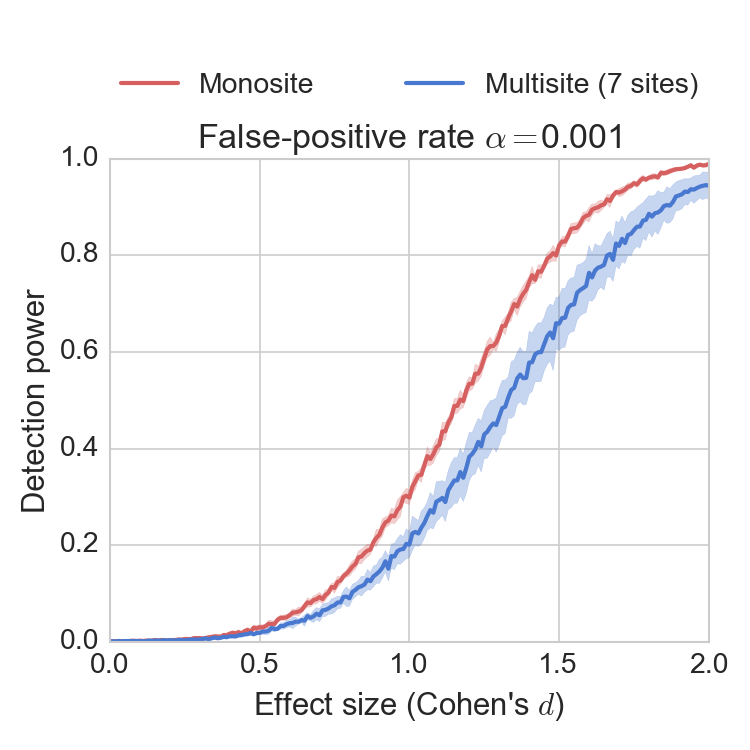
\includegraphics[width=0.32\textwidth]{../figures/realdata_detect_pow_s40_50pct.png}}
\hspace{1mm}
\subfloat[][80 subjects]{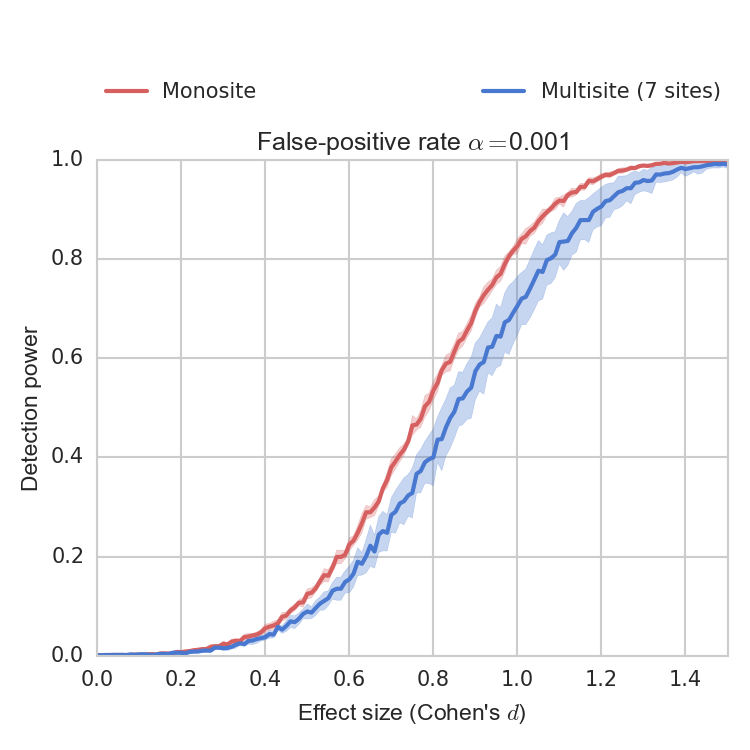
\includegraphics[width=0.32\textwidth]{../figures/realdata_detect_pow_s80_50pct.png}}
\hspace{1mm}
\subfloat[][120 subjects]{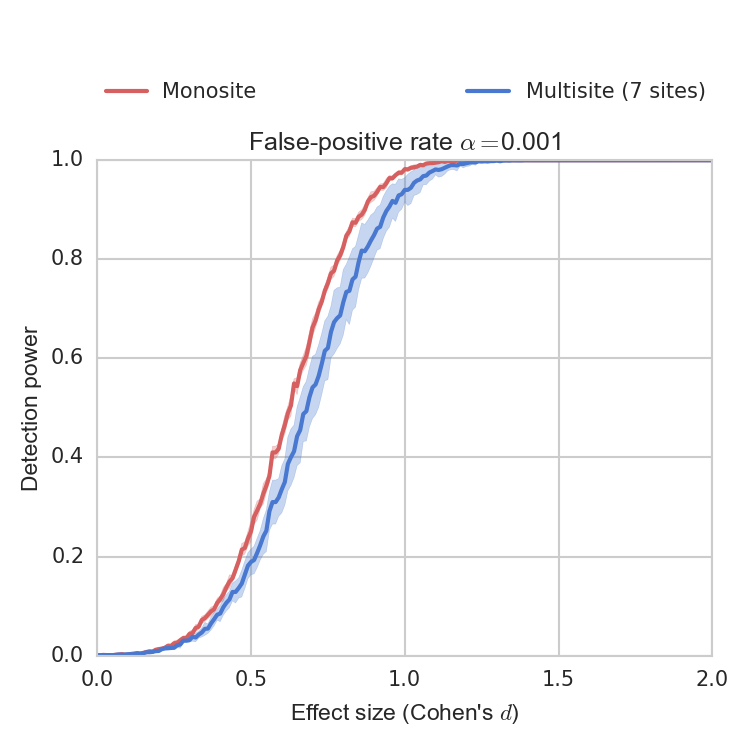
\includegraphics[width=0.32\textwidth]{../figures/realdata_detect_pow_s120_50pct.png}}
\hspace{1mm}
\caption{
Simulation on real data, detection power of two groups balanced 50\%-50\% between 7 sites. Two scenarios, 1) monosite and 2) multisite 7 sites with correction for multisite differences using dummy variables. Each plot show the detection power in function of the effect size for 3 different sample size 40, 80 and 120 subjects in total.
}
\label{fig_real_sim_samplesize}
\end{figure}

In Figure \ref{fig_sampeffect_curves_alpha001} show the sample-size in function of the effect-size for a detection power of 80\%. A threshold on the statistical power of each test is applied at three alpha values: 0.001, (see alpha of 0.01 and 0.05 in supplementary material \ref{fig_sampeffect_curves_alpha01},\ref{fig_sampeffect_curves_alpha01}). We are reporting the parametric curve and the points obtained using our simulations for the monosite and the multisite. As we can see the monosite is concordant with the parametric estimation and the multisite is offset of approximately 20 subjects more for the same effect-size.


\begin{figure}[tbp]
\centering
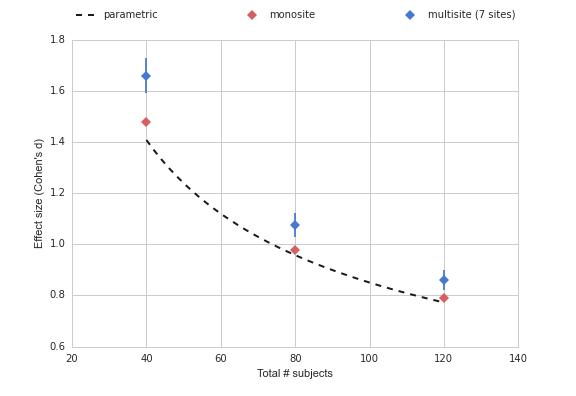
\includegraphics[width=0.5\textwidth]{../figures/samplesize_effectsize_pow80_alpha001.png}
\caption[]{
Sample-size in function of the effect-size for a detection power of 80\% and alpha of 0.001.
}
\label{fig_sampeffect_curves_alpha001}
\end{figure}


Figure \ref{fig_real_sim_debalancing} show the effect of debalancing the two groups at various ratio (50\%-50\% , 30\%-70\% and 15\%-85\%) for a total sample size of 120 subjects. Has the debalancing increase our ability to detect effect is diminished. As an example for an effect size of 1 we would detect the effect in 95\% of the cases in a 50 balanced scenario, this would go down to 90\% in a 30\%-70\% scenario and to 60\% in a 15\%-85\% debalancing. 


%\frametitle{Debalancing effect: \\real data 120 subjects total}
\begin{figure}[tbp]
\centering
\captionsetup[subfloat]{labelformat=empty}
\subfloat[][Debalancing 50\%]{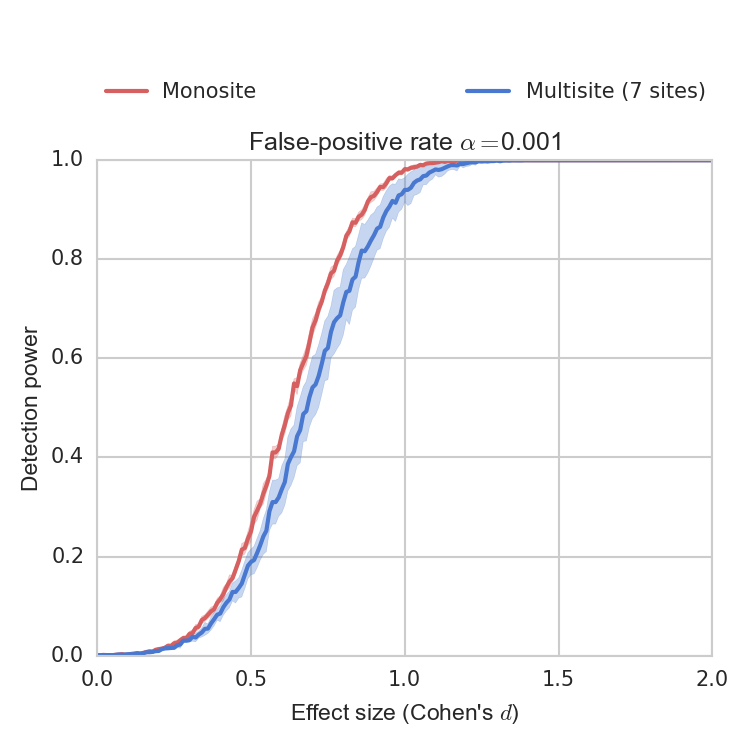
\includegraphics[width=0.32\textwidth]{../figures/realdata_detect_pow_s120_50pct.png}}
\hspace{1mm}
\subfloat[][Debalancing 30\%]{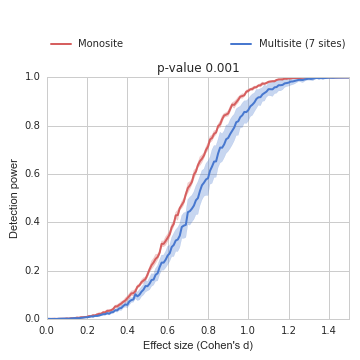
\includegraphics[width=0.32\textwidth]{../figures/realdata_detect_pow_s120_30pct.png}}
\hspace{1mm}
\subfloat[][Debalancing 15\%]{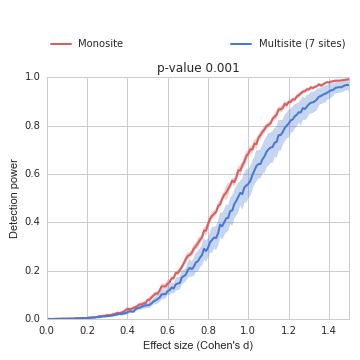
\includegraphics[width=0.32\textwidth]{../figures/realdata_detect_pow_s120_15pct.png}}
\hspace{1mm}
\caption{
Simulation on real data, detection power of two groups for a total of 120 subject between 7 sites. All plot show two scenarios, 1) monosite and 2) multisite 7 sites with correction for multisite differences using dummy variables.
}
\label{fig_real_sim_debalancing}
\end{figure}

Figure \ref{fig_real_sim_debalancing_interact} show the effect of debalancing the two groups at various ratio (50\%-50\% , 30\%-70\% and 15\%-85\%) with an interaction site-pathology (0.5 Cohen's d) for a total sample size of 120 subjects. Has the debalancing increase our ability to detect effect is diminished. As an example for an effect size of 1 we would detect the effect in 98\% of the cases in a 50 balanced scenario, this would go down to 95\% in a 30\%-70\% scenario and to 75\% in a 15\%-85\% debalancing. The particularity of this experiment is the fact that the multisite configuration perform better then the single site meanning that it is better to have interaction of various amplitude across small sites than an average interaction on one large site.


%\frametitle{Debalancing effect + interaction site-patho: \\real data 120 subjects total}
\begin{figure}[tbp]
\centering
\captionsetup[subfloat]{labelformat=empty}
\subfloat[][Debalancing 50\%]{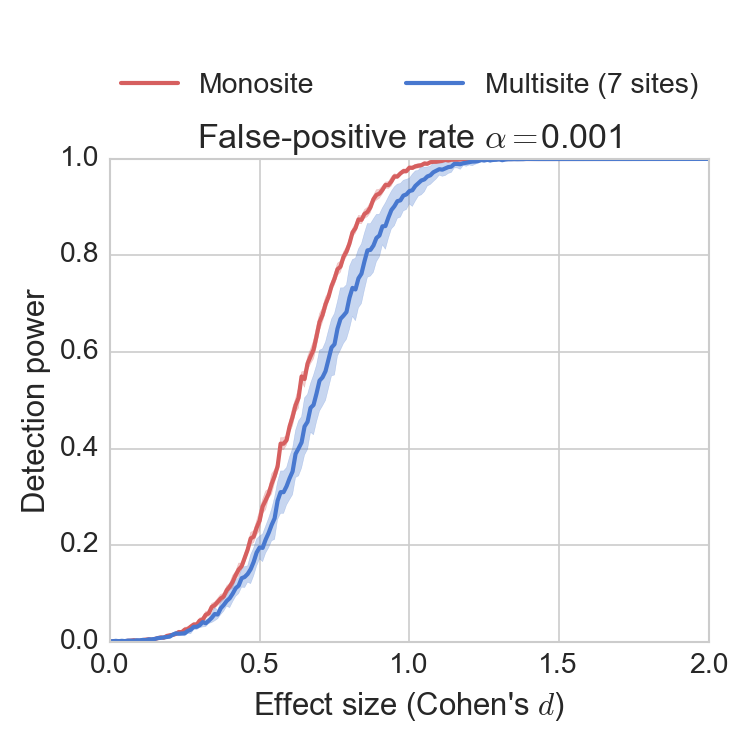
\includegraphics[width=0.32\textwidth]{../figures/realdata_detect_pow_sitepatho_s120_50pct.png}}
\hspace{1mm}
\subfloat[][Debalancing 30\%]{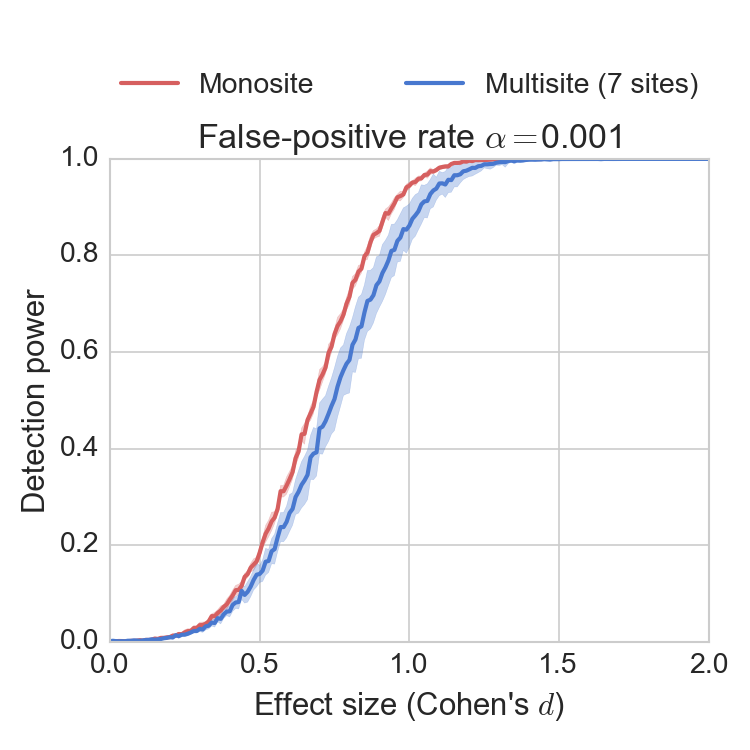
\includegraphics[width=0.32\textwidth]{../figures/realdata_detect_pow_sitepatho_s120_30pct.png}}
\hspace{1mm}
\subfloat[][Debalancing 15\%]{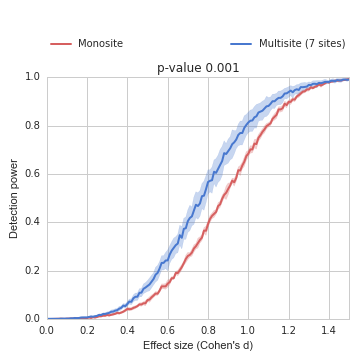
\includegraphics[width=0.32\textwidth]{../figures/realdata_detect_pow_sitepatho_s120_15pct.png}}
\hspace{1mm}
\caption{
Simulation on real data, detection power of two groups for a total of 120 subject between 7 sites with a site-pathology interaction at 0.5. All plot show two scenarios, 1) monosite and 2) multisite 7 sites with correction for multisite differences using dummy variables.
}
\label{fig_real_sim_debalancing_interact}
\end{figure}

Figure \ref{fig_real_sim_debalancing_2sites} show a scenario of two site one large (80 subjects) and one small ($\sim20$ subjects) unbalanced at 30\%-70\% and the inverse. As we can see the multisite configuration is as good as the monosite.

\begin{figure}[tbp]
\centering
\captionsetup[subfloat]{labelformat=empty}
\subfloat[\tiny 30\%-70\%]{\label{} 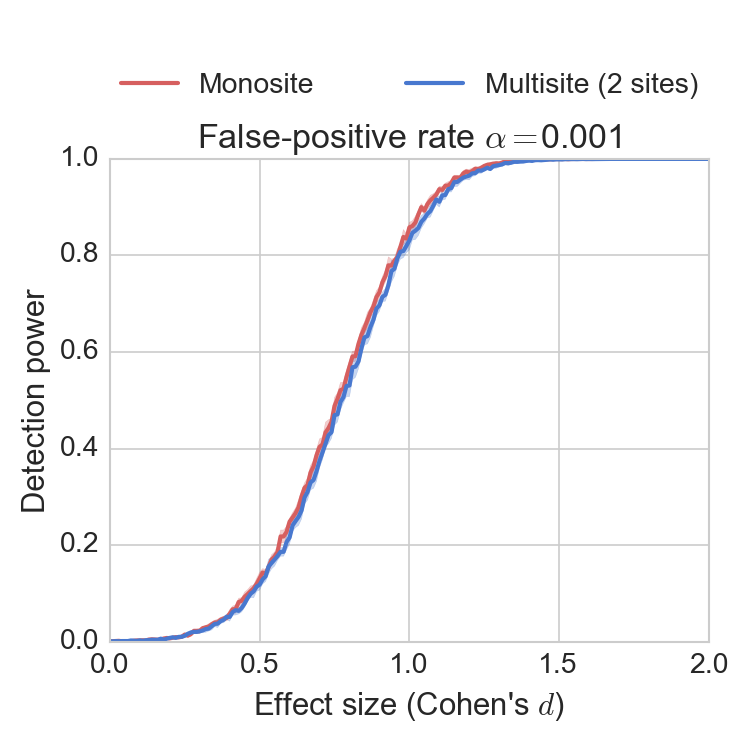
\includegraphics[width=0.39\textwidth]{../figures/realdata_detect_pow_sitepatho2site_s100_30pct.png}} 
\subfloat[\tiny 70\%-30\%]{\label{} 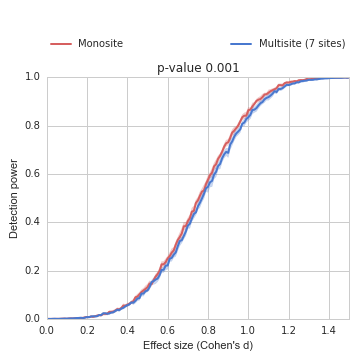
\includegraphics[width=0.39\textwidth]{../figures/realdata_detect_pow_sitepatho2site_s100_70pct.png}}\\
\caption{
Simulation on real data, detection power of two groups for a total of 100 subject between 2 sites, one small site of 20 subjects and one large of 80 subjects. All plot show two scenarios, 1) monosite and 2) multisite 2 sites with correction for multisite differences using dummy variables. Simulation of the detection power of two groups balanced 30\% and 70\% between 2 sites.
}
\label{fig_real_sim_debalancing_2sites}
\end{figure}

Using this Monte-Carlo simulations we have shown that the power of detecting an effect is marginally affected by the site acquisition configuration (single site or multi-site) when the sites are balanced in term of the amount of subject with and without the effect. 


\subsection{Simulation on synthetic data}
 
In order to obtain more control on each of the parameter of the simulation and simulate some configuration that were not possible to do with the real data (like the simulation of 2 medium size sites of of 40 and 60 subjects per site, and the size of the site effect) we have therefore used a synthetic model using only synthetic data and the average standard deviation of the Cambridge site connectivity. All plots show four scenarios: The top left plot represent the two configurations one monosite and two sites with correction for multisite differences using dummy variables without site effect. Has expected there is no difference between using 1 large site than combining two site of half the size. The plot on the upper right corner represent the detection power when we apply a site effect on balanced sites, here again not much differences an additive effect is fully compensated by the dummy variables corrective method. the lower left plot represent no site effect but an interaction between site and pathology. An the last plot on the lower right corner show the detection power with a site effect of 0.5 and a interation site pathology.

%\begin{frame} \frametitle{50-50 subjects, 50\%-50\% debalancing effect}
 \begin{figure}[tbp]
   \centering
    \captionsetup[subfloat]{labelformat=empty}
    \subfloat[]{ 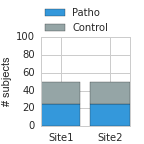
\includegraphics[width=0.19\textwidth]{../figures/prop_5050subj_5050.png}}
     \subfloat[\tiny No site effect]{ 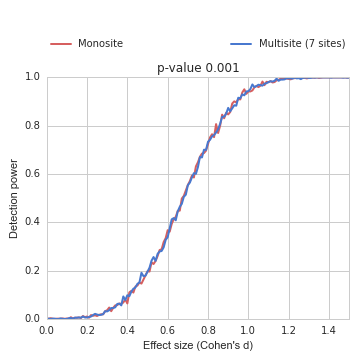
\includegraphics[width=0.39\textwidth]{../figures/detect_pow_bal5050_var0_site0.png}} 
     \subfloat[\tiny Site effect of 0.5]{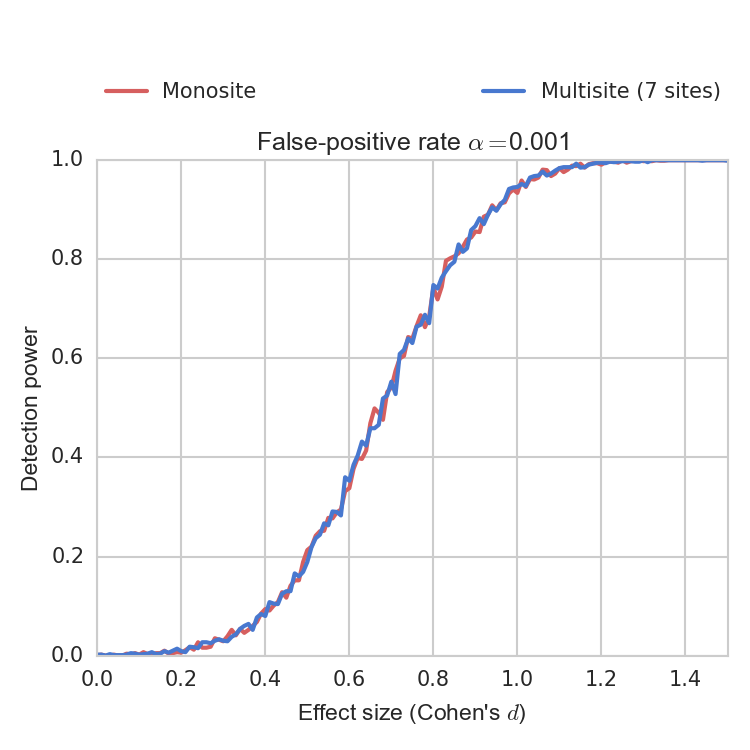
\includegraphics[width=0.39\textwidth]{../figures/detect_pow_bal5050_var0_site05.png}}\\[-2.7ex] 
     \hspace*{6.8em}
     \subfloat[\tiny Inter site-patho, no site effect]{ 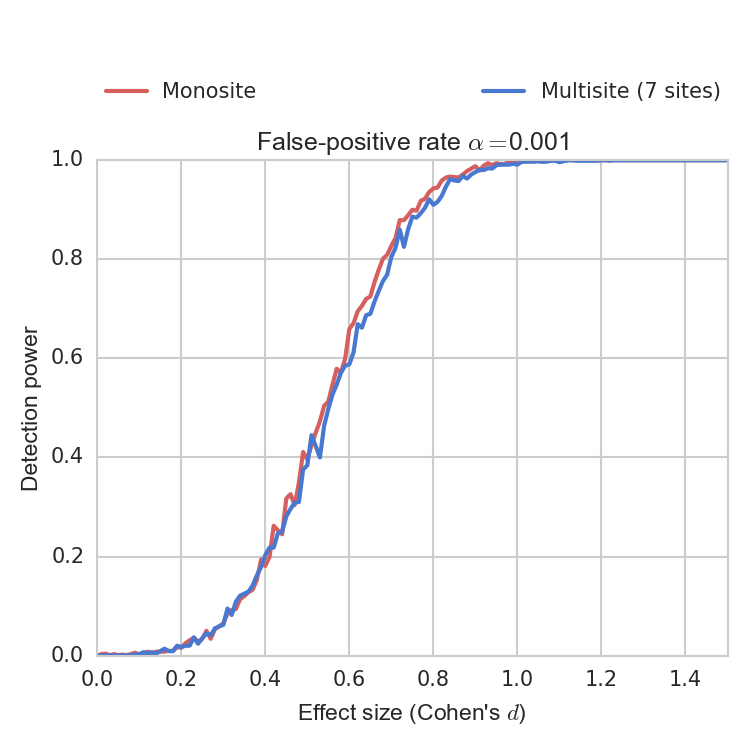
\includegraphics[width=0.39\textwidth]{../figures/detect_pow_bal5050_var2_site0.png}}
     \subfloat[\tiny Inter site-patho + site effect]{ 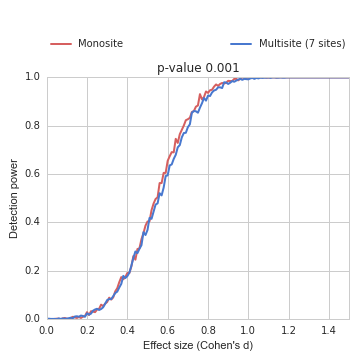
\includegraphics[width=0.39\textwidth]{../figures/detect_pow_bal5050_var2_site05.png}}\\
     \caption{
     Simulation of the detection power of two groups balanced 50\%-50\% between two sites. All plots show four scenarios in two configuration one monosite and two sites with correction for multisite differences using dummy variables. The first column represent scenarios without site effect and the second column show with a site effect the first row show simulation with out interaction site-pathology and the second row show with interaction.
}
\label{fig_full_sim_site_effect}
 \end{figure}
 

%
%\begin{frame} \frametitle{50-50 subjects, 70\%-30\% debalancing effect}
 \begin{figure}[tbp]
   \centering
    \captionsetup[subfloat]{labelformat=empty}
    \subfloat[]{ 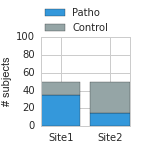
\includegraphics[width=0.19\textwidth]{../figures/prop_5050subj_7030.png}}
     \subfloat[\tiny No site effect]{\label{} 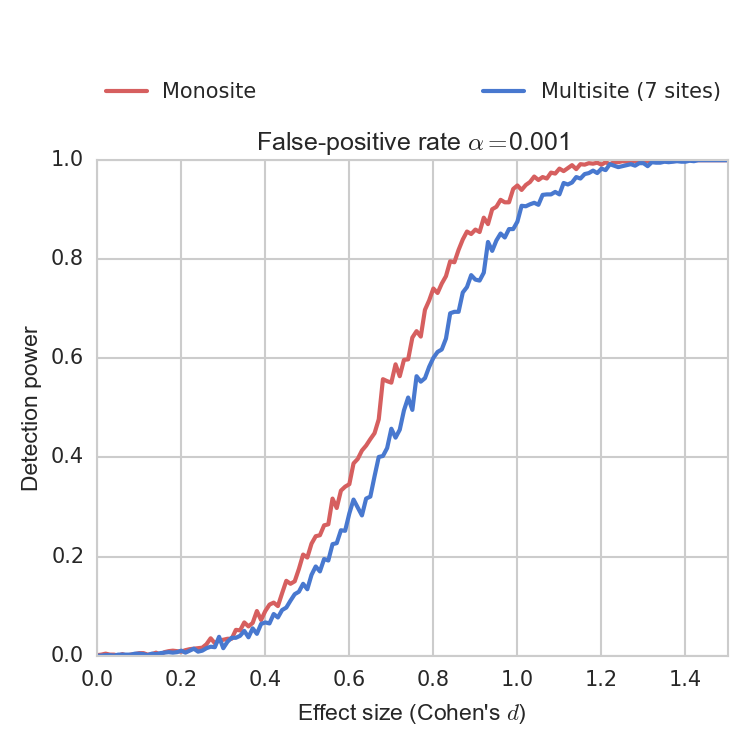
\includegraphics[width=0.39\textwidth]{../figures/detect_pow_bal7030_var0_site0.png}} 
     \subfloat[\tiny Site effect of 0.5]{\label{} 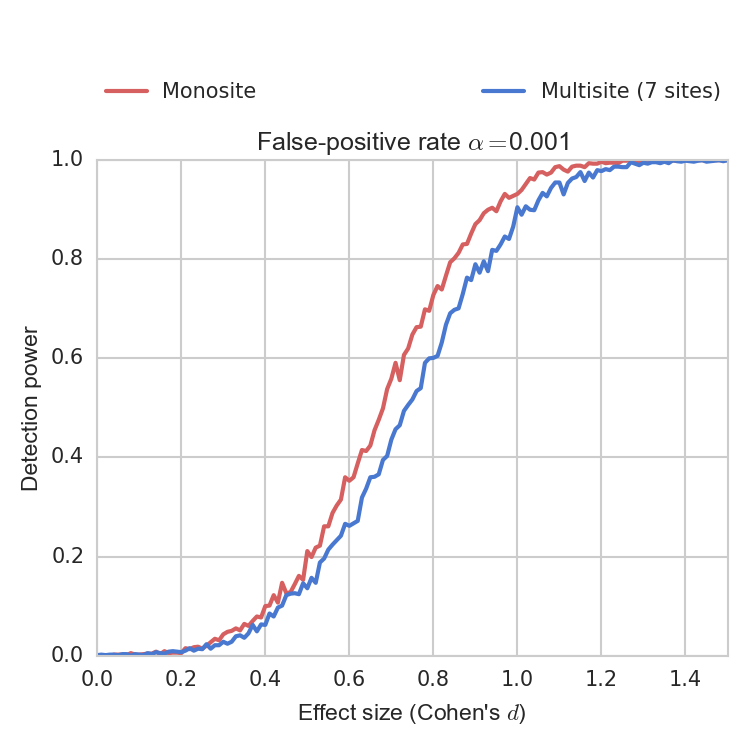
\includegraphics[width=0.39\textwidth]{../figures/detect_pow_bal7030_var0_site05.png}}\\[-2.7ex]
     \hspace*{6.8em}
     \subfloat[\tiny Interac site-patho, no site effect]{\label{} 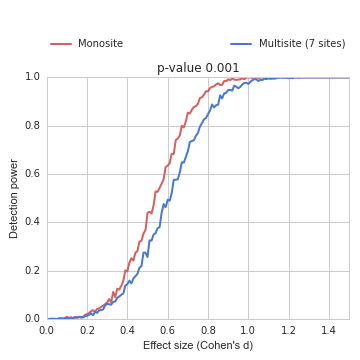
\includegraphics[width=0.39\textwidth]{../figures/detect_pow_bal7030_var2_site0.png}}
     \subfloat[\tiny Interac site-patho + site effect]{\label{} 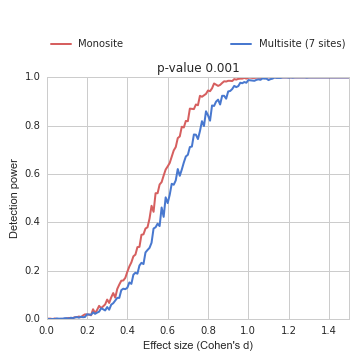
\includegraphics[width=0.39\textwidth]{../figures/detect_pow_bal7030_var2_site05.png}}\\
     \caption{
     Simulation of the detection power of two groups unbalanced 70\%-30\% between two sites. All plots show four scenarios in two configuration one monosite and two sites with correction for multisite differences using dummy variables. The first column represent scenarios without site effect and the second column show with a site effect the first row show simulation with out interaction site-pathology and the second row show with interaction.
}
     \label{fig_full_sim_debalancing}
 \end{figure}
 


%\frametitle{20-80 subjects, 50\%-50\% debalancing effect}
 \begin{figure}[tbp]
   \centering
    \captionsetup[subfloat]{labelformat=empty}
    \subfloat[]{ 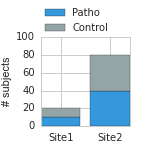
\includegraphics[width=0.19\textwidth]{../figures/prop_2080subj_5050.png}}
     \subfloat[\tiny No site effect]{\label{} 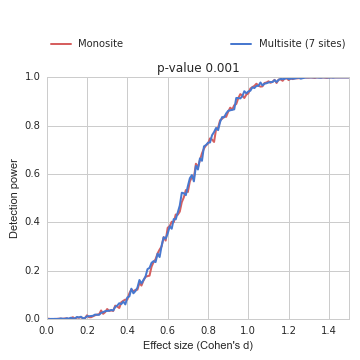
\includegraphics[width=0.39\textwidth]{../figures/detect_pow_2080bal5050_var0_site0.png}} 
     \subfloat[\tiny Site effect of 0.5]{\label{} 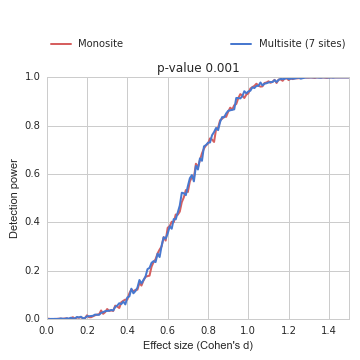
\includegraphics[width=0.39\textwidth]{../figures/detect_pow_2080bal5050_var0_site05.png}}\\[-2.7ex]
     \hspace*{6.8em}
     \subfloat[\tiny Interac site-patho, no site effect]{\label{} 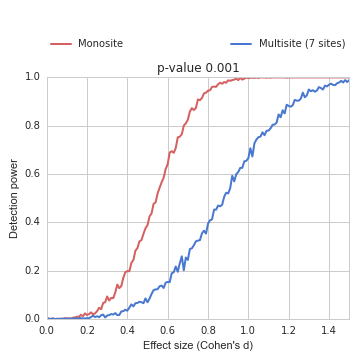
\includegraphics[width=0.39\textwidth]{../figures/detect_pow_2080bal5050_var2_site0.png}} 
     \subfloat[\tiny Interac site-patho + site effect]{\label{} 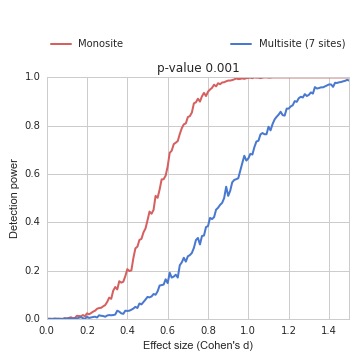
\includegraphics[width=0.39\textwidth]{../figures/detect_pow_2080bal5050_var2_site05.png}}\\
     \caption{
     Simulation of the detection power of two groups unbalanced 50\%-50\% between two sites, one small site of 20 subjects and one large of 80 subjects. All plots show four scenarios in two configuration one monosite and two sites with correction for multisite differences using dummy variables. The first column represent scenarios without site effect and the second column show with a site effect the first row show simulation with out interaction site-pathology and the second row show with interaction.
}
\label{fig_full_sim_2sites_balanced}
\end{figure}
 
Figure \ref{fig_full_sim_2sites_debalancing_inv} show the same configuration but the sample size are inverted. Has we can see we have the same pattern as in the real data with...

%\begin{frame} \frametitle{20-80 subjects, 70\%-30\% debalancing effect}
 \begin{figure}[tbp]
   \centering
    \captionsetup[subfloat]{labelformat=empty}
    \subfloat[]{ 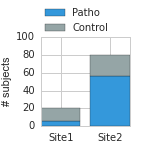
\includegraphics[width=0.19\textwidth]{../figures/prop_2080subj_7030.png}}
     \subfloat[\tiny No site effect]{\label{} 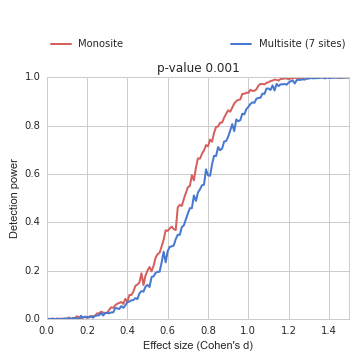
\includegraphics[width=0.39\textwidth]{../figures/detect_pow_2080bal7030_var0_site0.png}} 
     \subfloat[\tiny Site effect of 0.5]{\label{} 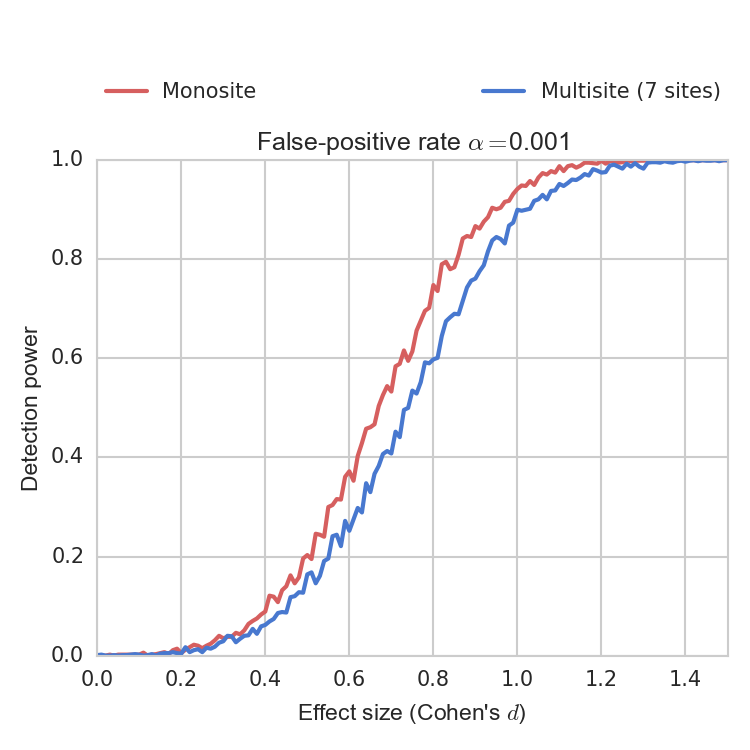
\includegraphics[width=0.39\textwidth]{../figures/detect_pow_2080bal7030_var0_site05.png}}\\[-2.7ex]
     \hspace*{6.8em}
     \subfloat[\tiny Interac site-patho, no site effect]{\label{} 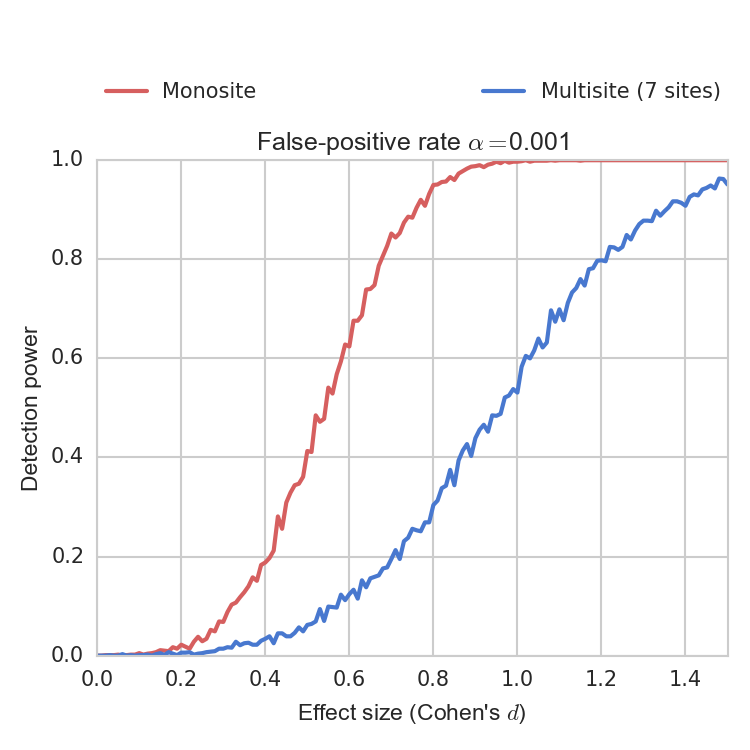
\includegraphics[width=0.39\textwidth]{../figures/detect_pow_2080bal7030_var2_site0.png}} 
     \subfloat[\tiny Interac site-patho + site effect]{\label{} 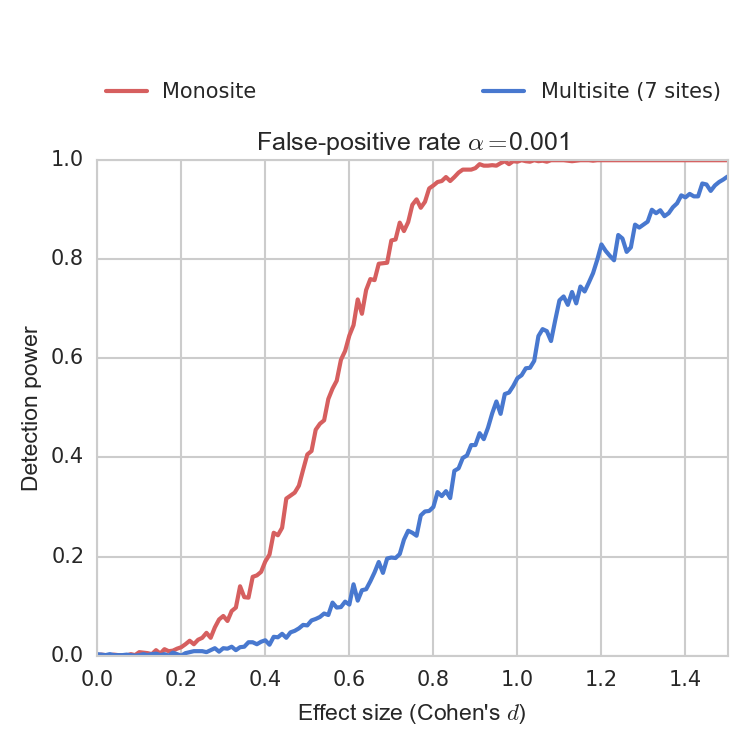
\includegraphics[width=0.39\textwidth]{../figures/detect_pow_2080bal7030_var2_site05.png}}\\
     \caption{
     Simulation of the detection power of two groups unbalanced 70\%-30\% between two sites, one small site of 20 subjects and one large of 80 subjects. All plots show four scenarios in two configuration one monosite and two sites with correction for multisite differences using dummy variables. The first column represent scenarios without site effect and the second column show with a site effect the first row show simulation with out interaction site-pathology and the second row show with interaction.
}
     \label{fig_full_sim_2sites_debalancing}
 \end{figure}
 
 


%\begin{frame} \frametitle{80-20 subjects, 70\%-30\% debalancing effect}
 \begin{figure}[tbp]
   \centering
    \captionsetup[subfloat]{labelformat=empty}
    \subfloat[]{ 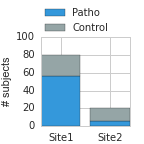
\includegraphics[width=0.19\textwidth]{../figures/prop_8020subj_7030.png}}
     \subfloat[\tiny No site effect]{\label{} 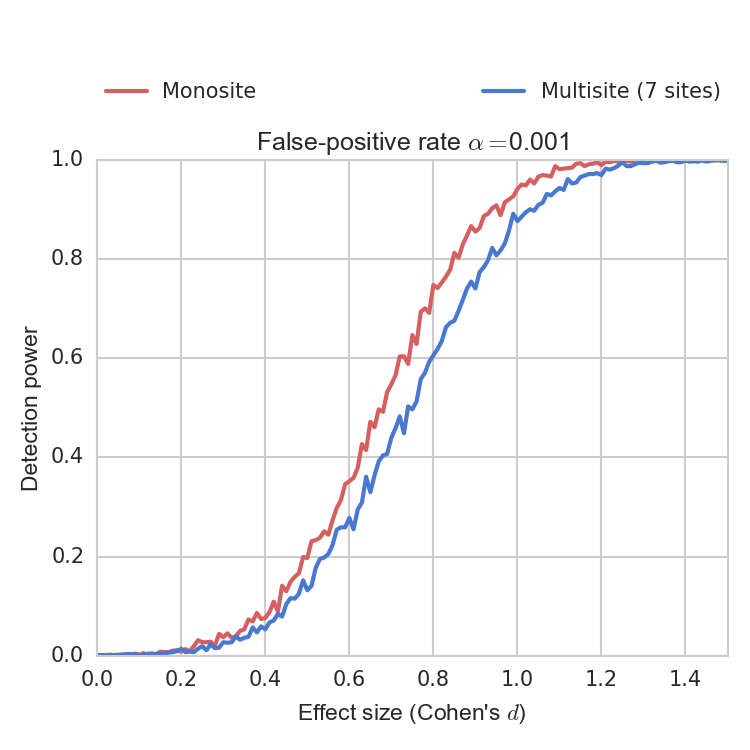
\includegraphics[width=0.39\textwidth]{../figures/detect_pow_8020bal7030_var0_site0.png}} 
     \subfloat[\tiny Site effect of 0.5]{\label{} 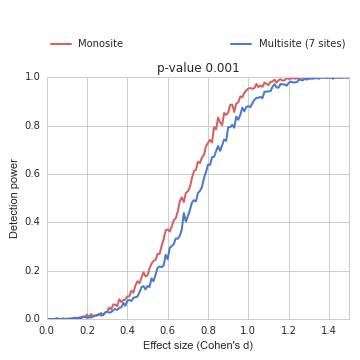
\includegraphics[width=0.39\textwidth]{../figures/detect_pow_8020bal7030_var0_site05.png}}\\[-2.7ex]
     \hspace*{6.8em}
     \subfloat[\tiny Interac site-patho, no site effect]{\label{} 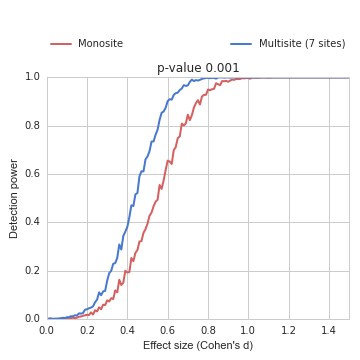
\includegraphics[width=0.39\textwidth]{../figures/detect_pow_8020bal7030_var2_site0.png}} 
     \subfloat[\tiny Interac site-patho + site effect]{\label{} 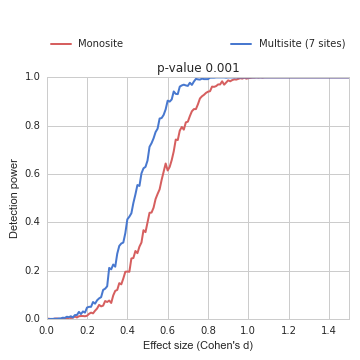
\includegraphics[width=0.39\textwidth]{../figures/detect_pow_8020bal7030_var2_site05.png}}\\
     \caption{
     Simulation of the detection power of two groups unbalanced 70\%-30\% between two sites, one small site of 20 subjects and one large of 80 subjects. All plots show four scenarios in two configuration one monosite and two sites with correction for multisite differences using dummy variables. The first column represent scenarios without site effect and the second column show with a site effect the first row show simulation with out interaction site-pathology and the second row show with interaction.
}
     \label{fig_full_sim_2sites_debalancing_inv}
 \end{figure}
 
Figure \ref{fig_full_sim_50sites_rnd_debalancing} show a more realistic case in clinical trials where the number of scanning sites is very large and the number of subjects per site is small. There is usually no control on the exact balancing of those sites therefore we have randomly assign debalancing for each site (between 10\% and 90\%) and have randomly assigned a number of subject to each site (between 2 and 15 subjects).

\begin{figure}[tbp]
   \centering
    \captionsetup[subfloat]{labelformat=empty}
     \subfloat[\tiny No interaction site-patho]{\label{} 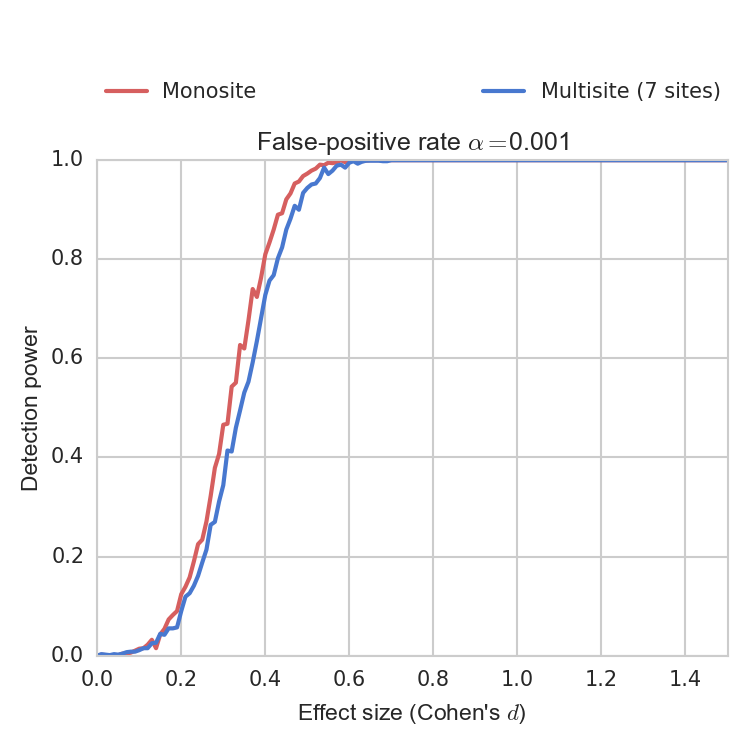
\includegraphics[width=0.39\textwidth]{../figures/detect_pow_rndsubj0215_50sites_rndbal1090_var0_siternd0005.png}} 
     \subfloat[\tiny Site effect of 0.5]{\label{} 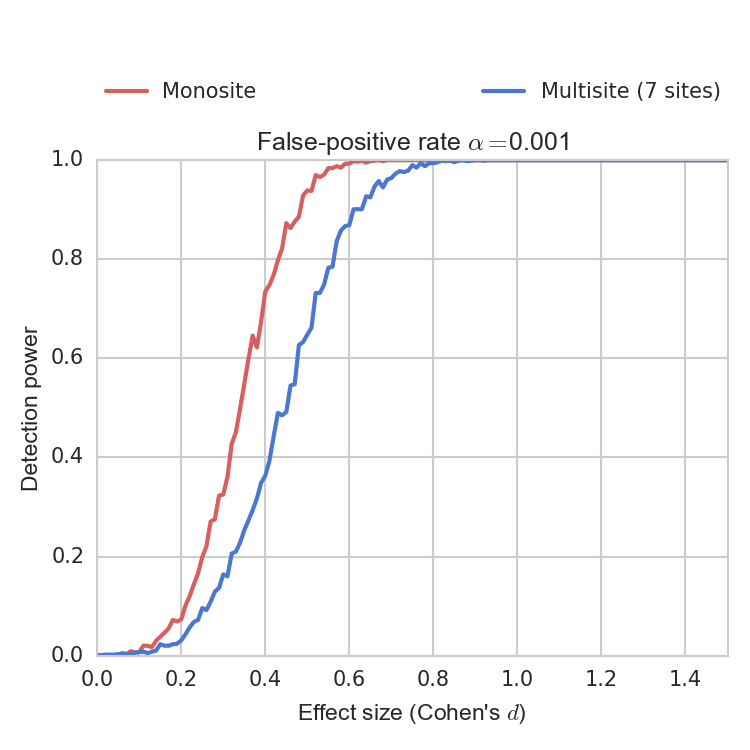
\includegraphics[width=0.39\textwidth]{../figures/detect_pow_rndsubj0215_50sites_rndbal1090_varrnd02_siternd0005.png}}\\
     \caption{
     Simulation of the detection power of two groups balanced randomly between 10\%-90\% between 50 sites, the number of subject per site is randomly assigned between 2 and 15. All plot show two scenarios, one monosite and two sites with correction for multisite differences using dummy variables. The plots show the detection power when the variability is greater in one side then the other for the pathology group (twice the reference variability in one site and half the reference variability in the other one).
}
     \label{fig_full_sim_50sites_rnd_debalancing}
\end{figure}

\section{Discussion}

Connectivity bias that can impact interpretation.\\

Type of scanner most of them are Siemens we may have more variability if combining various brand\\


Talk about the impact in small acquisition 40 subjects total and the importance of pooling data among PI.\\
Choosing the right sample size for a given detection power to obtain reproducible results.

Talk about the impact in clinical trial and best practice.\\
	most of the time we cannot correct for site with one population only or with too few subjects per site. Although these kind of multisite studies generally sum-up to large dataset of more than 200 subjects. has we demonstrated in the synthetic simulation such configuration are comparable to single site analysis for this range of sample size.

It is better to have interaction of various amplitude across small sites than an average interaction on one large site\\

talk about the reduction of the bias of the simulation compared to the fully parametric estimate as we increase the sample size. The estimation is more realistic over 80 subjects and overestimate the detection power at low sample-size.

% can be use for other multisite study...
Despite justifiable scepticism, feasibility analyses demonstrated that meaningful explorations of the aggregate dataset, composed of 24 imaging sites for a grand total of 1093 subjects, could be performed \citep{Biswal2010}. Although no explicit correction for multi-site variability was used, they only use global signal correction (GSC) to normalize subjects which may introduce anti-correlation in the data \citep{Fox2009, Murphy2009, Saad2012, Carbonell2014, Power2014}. After accounting for site-related differences, the analysis showed brain-behaviour relationships with phenotypic variables such as age, gender, and diagnostic label, and confirmed a variety of prior hypotheses \citep{Biswal2010, Fair2012, Tomasi2010, Zuo2012}. While encouraging, many uncontrolled and unknown factors in the 1000 FCP remain a source of concern, as they spread beyond simple site effects and can limit the datasets utility as highlighted by \cite{Yan2013}. Another compelling proof of multisite bias is the study reported by \cite{Nielsen2013} where they did an analysis on a single site dataset and a multi-site dataset of subject with autism and concluded that the multi-site autism study classification accuracy significantly outperformed chance but was much lower for multi-site prediction than for previous single site results \citep{Nielsen2013}. We therefore need to keep in mind that the site effect must be taken in account in the analysis or we may reduce our detection power.

\section{Conclusion}


\section{Acknowledgments}
Parts of this work were presented at the 2013 annual meetings of the organization for human brain mapping \citep{Dansereau2013a}, as well as the  Alzheimer's Association International Conference (AAIC) (2013) (Boston) \citep{Dansereau2013b}. The authors are grateful to the members of the 1000 functional connectome consortium for publicly releasing there dataset. The computational resources used to perform the data analysis were provided by ComputeCanada\footnote{\url{https://computecanada.org/}} and CLUMEQ\footnote{\url{http://www.clumeq.mcgill.ca/}}, which is funded in part by NSERC (MRS), FQRNT, and McGill University. This project was funded by NSERC grant number RN000028, a salary award from ``Fonds de recherche du Qu\'ebec -- Sant\'e'' to PB as well as a salary award by the Canadian Institute of Health Research to CD.

\section*{References}

\bibliographystyle{elsarticle-harv}
\bibliography{cdansereau}


\pagebreak



\clearpage
\appendix


%% SUPPLEMENTARY MATERIAL
\clearpage
\pagebreak
\renewcommand{\thefigure}{S\arabic{figure}}
\renewcommand{\thetable}{S\arabic{table}}
\setcounter{figure}{0}
\begin{center}
\emph{Supplementary Material {--} Feasibility of multi-centric fMRI connectivity studies of Alzheimer's disease}\\

\vspace{\baselineskip}Submitted to Neuroimage.\\

\vspace{\baselineskip}C. Dansereau$^{1,2}$,  C. Risterucci$^{3}$, E. Merlo Pich$^{3}$, D. Arnold$^{4}$, P. Bellec$^{1,2}$\\

\end{center}
$^1$Functional Neuroimaging Unit, Centre de Recherche de l'Institut Universitaire de G\'eriatrie de Montr\'eal\\
$^2$Department of Computer Science and Operations Research, University of Montreal, Montreal, Quebec, Canada\\
$^3$F. Hoffmann-La Roche Ldt., Basel, Switzerland\\
$^4$NeuroRx, Montreal, Quebec, Canada\\

For all questions regarding the paper, please address correspondence to Pierre Bellec, CRIUGM, 4545 Queen Mary, Montreal, QC, H3W 1W5, Canada. Email: pierre.bellec (at) criugm.qc.ca.\\

\section*{Literature review: Alzheimer’s disease and resting-state fMRI} 
\begin{itemize}
\item \cite{Zhang2009a} used functional connectivity maps with a seed in the posterior cingulate cortex (PCC) to explore the differences between a group of elderly cognitively normal subjects (CNE, n=16) and patients with a mild dementia of the Alzheimer’s type (DAT, n=18).

\item \cite{Zhang2010} generalized the \cite{Zhang2009a} study with CNE (n=16) and a larger group of patients with DAT (n=46). Patients were separated in three groups (mild, moderate, severe DAT), and each group of patients was contrasted against the CNE.
\item \cite{Wang2006a} used functional connectivity maps with a seed in the hippocampi to explore the differences between a group of CNE (n=13) and patients with a mild DAT (n=13). All results included in the meta-analysis are from Table 2, seeded in the right hippocampus. Seeds were manually delineated on an individual basis.
\item \cite{Wang2007a} used functional connectivity maps with a seed in the posterior cingulate cortex (PCC) as well as full brain point-to-point correlations (based on an AAL parcellation) to explore the differences between a group of elderly cognitively normal subjects (CNE, n=14) and patients with a very mild to mild dementia of the Alzheimer’s type (DAT, n=14). Only the results based on the PCC seed were included in the meta-analysis.
\item \cite{Goveas2011} used functional connectivity maps with a seed in the hippocampi to explore the differences between a group of elderly cognitively normal subjects (CNE, n=18) and patients with a mild dementia of the Alzheimer’s type (DAT, n=14) before and after donepezil treatment. Seeds were manually delineated on an individual basis, before and after treatment.
\item \cite{Damoiseaux2012} used dual-regression independent component analysis to explore longitudinal differences between a group of CNE (n=18) and patients with DAT (n=21). All results included in the meta-analysis are from Table 3 (differences at baseline) and Table 4 (interaction with time). The authors used three components representing the Anterior DMN, Ventral DMN and Posterior DMN.
\end{itemize}


\pagebreak


\begin{figure}[tbp]
\centering
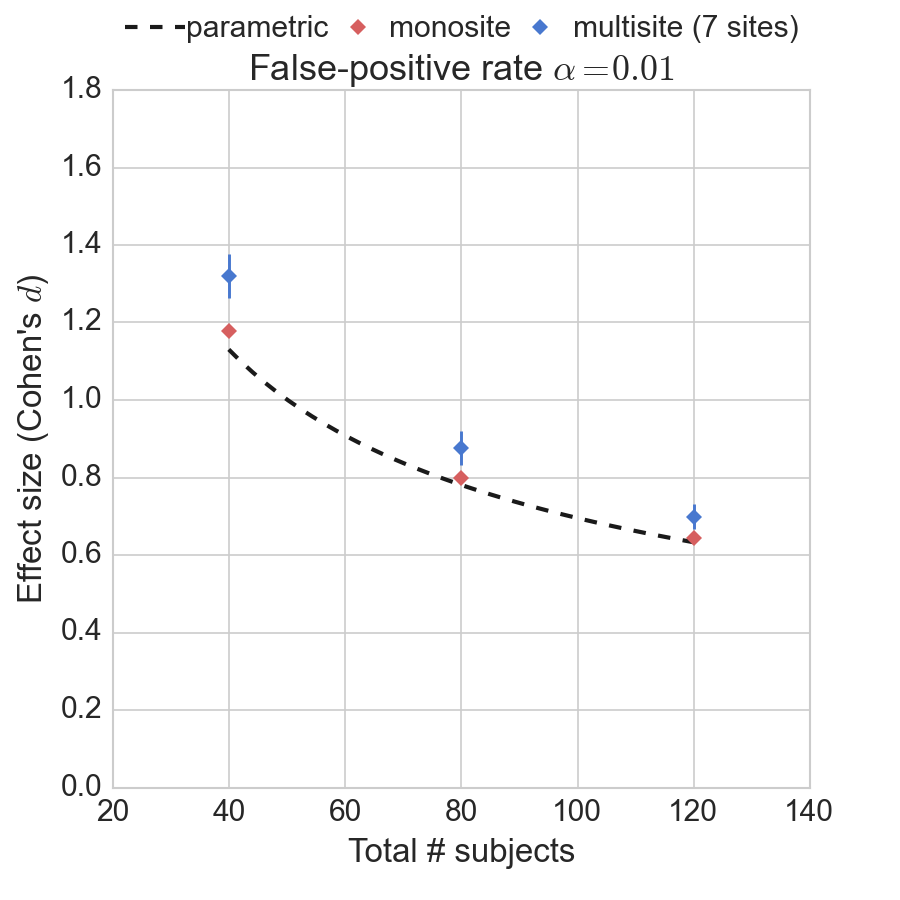
\includegraphics[width=0.32\textwidth]{../figures/samplesize_effectsize_pow80_alpha01.png}
\caption[]{
Sample-size in function of the effect-size for a detection power of 80\% and alpha of 0.001.
}
\label{fig_sampeffect_curves_alpha01}
\end{figure}
\begin{figure}[tbp]
\centering
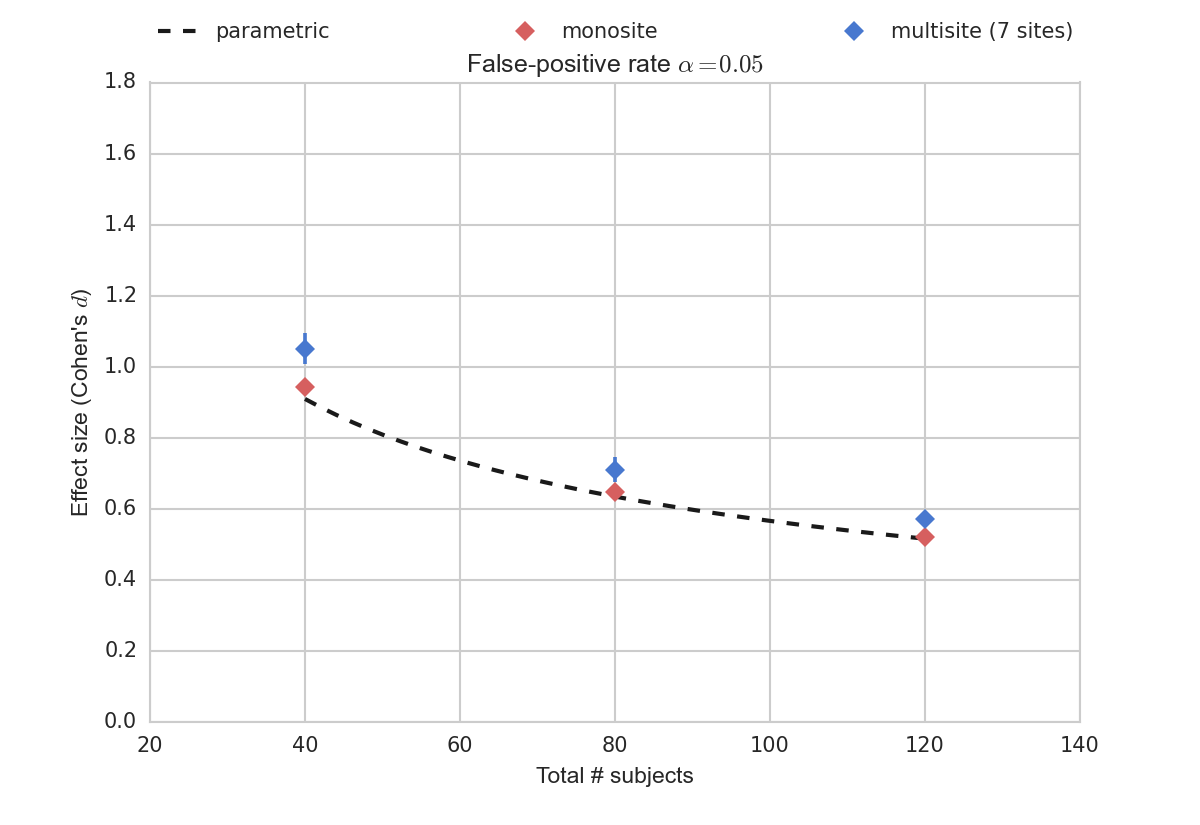
\includegraphics[width=0.32\textwidth]{../figures/samplesize_effectsize_pow80_alpha05.png}
\caption[]{
Sample-size in function of the effect-size for a detection power of 80\% and alpha of 0.001.
}
\label{fig_sampeffect_curves_alpha05}
\end{figure}

\end{document}


